%%%%%%%%%%%%%%%%%%%%%%%%%%%%%%%%%%%%%%%%%%%%%%%%%%%%%%%%%%%%%%%%%%%%%%%%%%%%%%%
\chapter{Oscilações}
\label{Chap:ExpOscilacoes}
%%%%%%%%%%%%%%%%%%%%%%%%%%%%%%%%%%%%%%%%%%%%%%%%%%%%%%%%%%%%%%%%%%%%%%%%%%%%%%%

\begin{fullwidth}\it
	Verificaremos o comportamento oscilatório de dois sistemas, um sistema massa-mola e um pêndulo simples. Veremos que através das Leis de Newton, chegamos a uma equação cuja solução é uma função periódica que descreve o movimento oscilatório observado. Utilizaremos os seguintes conceitos/técnicas de análise de dados: medidas, algarismos significativos, gráficos, erros de escala e propagados, equação geral para o erro propagado, regressão linear, e linearização,.
\end{fullwidth}

%%%%%%%%%%%%%%%%%%%%%%%%%%%%%%%%%%%%%%%%%%%%%%%%%%%%%%%%%%%%%%%%%%%%%%%%%%%%%%%
\section{Sistema massa-mola}
%%%%%%%%%%%%%%%%%%%%%%%%%%%%%%%%%%%%%%%%%%%%%%%%%%%%%%%%%%%%%%%%%%%%%%%%%%%%%%%

Sabemos que a força exercida por uma mola é proporcional à sua distensão:
\begin{align}
	F &= -k\Delta x \\
	&= -kx,
\end{align}
%
onde assumimos que $x_i = 0$ e $x_f = x$, que $k$ é uma constante de proporcionalidade, e onde o sinal negativo significa que a força é no sentido contrário à distensão da mola.

\begin{marginfigure}
	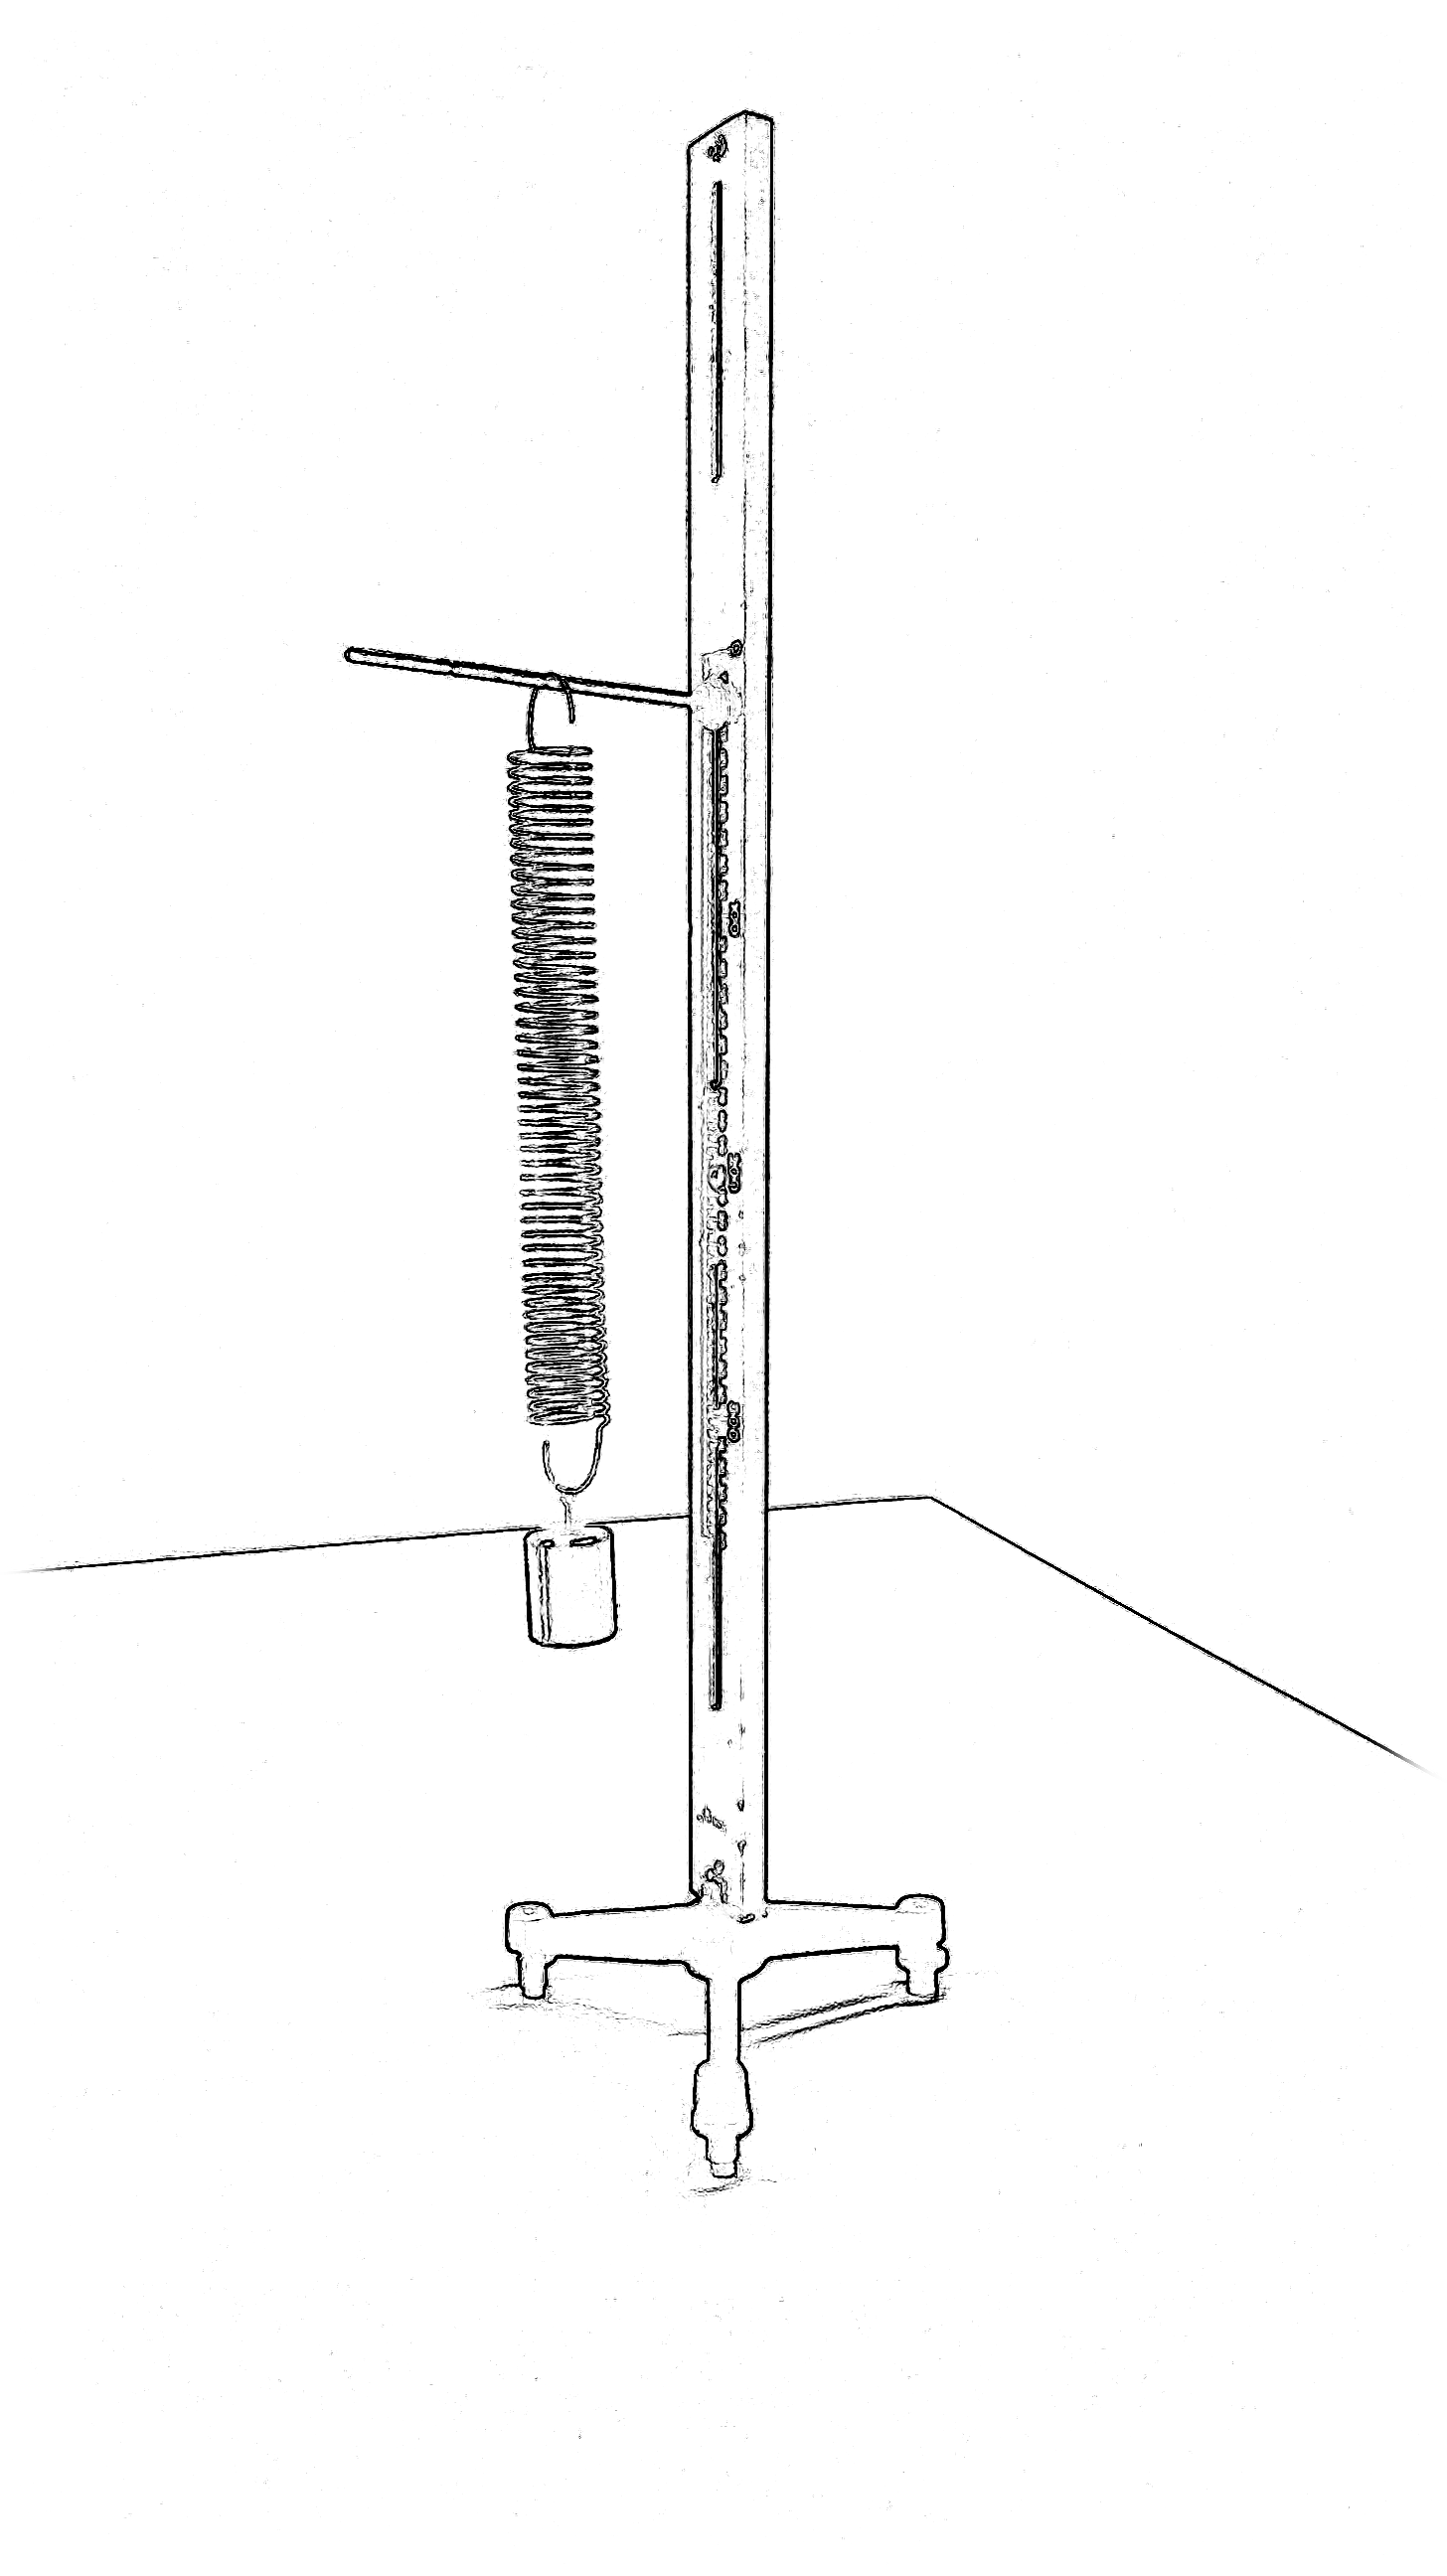
\includegraphics[width=\textwidth]{Ilustrations/Massa-Mola.png}
	\caption{Sistema massa-mola.}
\end{marginfigure}

\begin{marginfigure}
\centering
\begin{tikzpicture}[>=Stealth,
     interface/.style={
        % superfície
        postaction={draw,decorate,decoration={border,angle=-45,
                    amplitude=0.2cm,segment length=2mm}}},
    ]
    
    \draw[interface] (1,0) -- (-1,0);
    
    \draw (0,0) -- (0,-0.2);
    \draw[gray,decoration={aspect=0.3, segment length=1.5mm, amplitude=2mm,coil},decorate] (0,-0.2) -- +(0,-2);
    \draw (0,-2.2) -- (0,-2.4);
    
    \draw[pattern = north west lines] (-0.5, -2.4) rectangle (0.5,-3.4);
    
    \draw[fill] (0,-2.9) circle (1pt);
    \draw[->, thick] (0, -2.9) -- +(0,-1) node[right]{$\vec{P}$};
    \draw[->, thick] (0, -2.4) -- +(0,1) node[right]{$\vec{F}_e$};
    
    \draw[<-] (1,-1.9)node[below right]{$x$} -- (1,-3.9);
\end{tikzpicture}
\caption{Direção e sentido das forças em um sistema massa-mola.\label{Fig:BlocoEquilDevidoForcaElastica}}
\end{marginfigure}

Vamos considerar um sistema onde penduramos uma mola em um suporte, de forma que ela se disponha verticalmente, e prendemos um corpo de massa $m$ à extremidade inferior. Deixamos o corpo descer até que a força exercida pela mola equilibre o peso. A partir dessa posição de equilíbrio, qualquer deslocamento exercido fará com que atue sobre o corpo uma força proporcional ao deslocamento, porém com sentido contrário a ele, tendendo a restaurá-lo à posição de equilíbrio. Utilizando a segunda lei de Newton, podemos descrever a dinâmica do corpo através de
\begin{align}
    F_R^x &= m a_x \\
	P^x + F_e^x &= ma_x \\
	-P + (-kx) &= m a_x \\
	-k \left(x + \frac{mg}{k}\right) &= ma_x \\
	-kx' &= ma_x,
\end{align}
%
onde o eixo $x$ aponta verticalmente para cima e $x' \equiv x + mg/k$. A constante $mg/k$ na expressão acima representa a distensão da mola em relação à posição de equilíbrio. Note também que
\begin{align}
    a_x &= \frac{d^2}{dt^2}x \\
    a'_x &= \frac{d^2}{dt^2}x',
\end{align}
%
porém
\begin{align}
    a'_x &= \frac{d}{dt} x' \\
    &= \frac{d}{dt} \left(x - \frac{mg}{k}\right) \\
    &= \frac{d}{dt}x \\
    &= a_x,
\end{align}
%
pois $m$, $g$, e $k$ são constantes. Logo, podemos escrever
\begin{equation}
    -kx' = m a'_x,
\end{equation}
%
o que representa uma expressão para a aceleração em função da distensão da mola em relação à posição de equilíbrio do corpo.

Analisando essa equação, temos que sempre que o corpo se distancia da posição de equilíbrio, ele está sujeito a uma força na mesma direção, porém com o sentido oposto ao desse deslocamento, acelerando-o em direção à posição de em que a distensão da mola é nula (ou seja, em direção à posição de equilíbrio); isso é o que ocorre em todas as posições representadas na Figura~\ref{Fig:BlocoOscilando}, exceto $t_0$, $t_4$, e $t_7$. Quando o objeto passa pela posição de equilíbrio ---~posições $t_0$, $t_4$, e $t_7$~---, sua aceleração é zero, porém sua velocidade não, o que o faz com que ele continue o movimento, dando origem a um \emph{movimento oscilatório}.

Para descrever esse movimento, podemos substituir a aceleração na equação acima por sua definição em termos da derivada segunda da posição em relação ao tempo:
\begin{equation}
	-kx' = m\frac{d^2x'}{dt^2},
\end{equation}
%
ou, rearranjando os termos,
\begin{equation}\label{Eq:EquacaoDiferencialOHS}
	\frac{d^2x'}{dt^2} + \frac{k}{m} x' = 0.
\end{equation}

\begin{figure*}[b]
\centering
\begin{tikzpicture}[>=Stealth, scale = 0.75,
     interface/.style={
        % superfície
        postaction={draw,decorate,decoration={border,angle=-45,
                    amplitude=0.2cm,segment length=2mm}}},
    ]
    
    \draw[interface] (1,0) -- (-1,0);
    
    \draw (0,0) -- (0,-0.2);
    \draw[gray,decoration={aspect=0.3, segment length=1.55mm, amplitude=1.5mm,coil},decorate] (0,-0.2) -- +(0,-2);
    \draw (0,-2.2) -- (0,-2.4);
    
    \draw[pattern = north west lines] (-0.5, -2.4) rectangle (0.5,-3.4);
    
    \draw[fill] (0.7,-2.9) circle (1pt);
    \draw[->] (0.7,-2.9) -- node[right]{$\vec{v}$} +(0, -1);
    
    \draw[fill] (0,-2.9) circle (1pt);
    \draw[->, thick] (0, -2.9) -- +(0,-1) node[right]{$\vec{P}$};
    \draw[->, thick] (0, -2.4) -- +(0,1) node[right]{$\vec{F}_e$};
    
    \draw[dotted] (-1,-2.9) -- (20.2,-2.9);
    \draw[->] (-1,-5.9) -- (20.2,-5.9) node[below left]{$t$};
    
    \draw[->] (-1,-1.4) -- (-1,-4.4) node[above left]{$x$};
    \draw[|-] (-1,-2.9) node[left]{0} -- (-1,-4.4);
    \draw[|-|] (0,-5.9) node[below]{$t_0$} -- (2.4,-5.9) node[below]{$t_1$};
    \draw[|-|] (4.8,-5.9) node[below]{$t_2$} -- (7.2,-5.9) node[below]{$t_3$};
    \draw[|-|] (9.6,-5.9) node[below]{$t_4$} -- (12,-5.9) node[below]{$t_5$};
    \draw[|-|] (14.4,-5.9) node[below]{$t_6$} -- (16.8,-5.9) node[below]{$t_7$};
    \draw[-|] (16.8,-5.9) -- (19.2, -5.9) node[below]{$t_7$};
    
    \begin{scope}[shift={(2.4,0)}]
        \draw[interface] (1,0) -- (-1,0);
    
        \draw (0,0) -- (0,-0.2);
        \draw[gray,decoration={aspect=0.3, segment length=2.2mm, amplitude=1.5mm,coil},decorate] (0,-0.2) -- +(0,-3);
        \draw (0,-3.2) -- (0,-3.4);
        
        \draw[pattern = north west lines] (-0.5, -3.4) rectangle (0.5,-4.4);

        \draw[fill] (0.7,-3.9) circle (1pt);
        \draw[->] (0.7,-3.9) -- node[right]{$\vec{v}$} +(0, -0.75);
        \draw[->] (0.7, -3.9) -- node[right]{$\vec{a}$} +(0, 0.5);
        
        \draw[fill] (0,-3.9) circle (1pt);
        \draw[->, thick] (0, -3.9) -- +(0,-1) node[right]{$\vec{P}$};
        \draw[->, thick] (0, -3.4) -- +(0,1.3) node[right]{$\vec{F}_e$};
    \end{scope}
    
    \begin{scope}[shift={(4.8,0)}]
        \draw[interface] (1,0) -- (-1,0);
    
        \draw (0,0) -- (0,-0.2);
        \draw[gray,decoration={aspect=0.3, segment length=2.55mm, amplitude=1.5mm,coil},decorate] (0,-0.2) -- +(0,-3.5);
        \draw (0,-3.7) -- (0,-3.9);
        
        \draw[pattern = north west lines] (-0.5, -3.9) rectangle (0.5,-4.9);
        
        \draw[fill] (0.7,-4.4) circle (1pt);
        \draw[->] (0.7, -4.4) -- node[right]{$\vec{a}$} +(0, 0.75);
        
        \draw[fill] (0,-4.4) circle (1pt);
        \draw[->, thick] (0, -4.4) -- +(0,-1) node[right]{$\vec{P}$};
        \draw[->, thick] (0, -3.9) -- +(0,1.6) node[right]{$\vec{F}_e$};
    \end{scope}
    
    \begin{scope}[shift={(7.2,0)}]
        \draw[interface] (1,0) -- (-1,0);
    
        \draw (0,0) -- (0,-0.2);
        \draw[gray,decoration={aspect=0.3, segment length=2.2mm, amplitude=1.5mm,coil},decorate] (0,-0.2) -- +(0,-3);
        \draw (0,-3.2) -- (0,-3.4);
        
        \draw[pattern = north west lines] (-0.5, -3.4) rectangle (0.5,-4.4);
        
        \draw[fill] (0.7,-3.9) circle (1pt);
        \draw[->] (0.7,-3.9) -- node[above right]{$\vec{v}$} +(0, 0.75);
        \draw[->] (0.7, -3.9) -- node[right]{$\vec{a}$} +(0, 0.5);
        
        \draw[fill] (0,-3.9) circle (1pt);
        \draw[->, thick] (0, -3.9) -- +(0,-1) node[right]{$\vec{P}$};
        \draw[->, thick] (0, -3.4) -- +(0,1.3) node[right]{$\vec{F}_e$};
    \end{scope}
    
    %%% Meio
    \begin{scope}[shift={(9.6,0)}]
        \draw[interface] (1,0) -- (-1,0);
    
        \draw (0,0) -- (0,-0.2);
        \draw[gray,decoration={aspect=0.3, segment length=1.55mm, amplitude=1.5mm,coil},decorate] (0,-0.2) -- +(0,-2);
        \draw (0,-2.2) -- (0,-2.4);
        
        \draw[pattern = north west lines] (-0.5, -2.4) rectangle (0.5,-3.4);
        
        \draw[fill] (0.7,-2.9) circle (1pt);
        \draw[->] (0.7,-2.9) -- node[right]{$\vec{v}$} +(0, 1);
        
        \draw[fill] (0,-2.9) circle (1pt);
        \draw[->, thick] (0, -2.9) -- +(0,-1) node[right]{$\vec{P}$};
        \draw[->, thick] (0, -2.4) -- +(0,1) node[right]{$\vec{F}_e$};
    \end{scope}
    
    \begin{scope}[shift={(12.0,0)}]
        \draw[interface] (1,0) -- (-1,0);
    
        \draw (0,0) -- (0,-0.2);
        \draw[gray,decoration={aspect=0.3, segment length=0.8mm, amplitude=1.5mm,coil},decorate] (0,-0.2) -- +(0,-1);
        \draw (0,-1.2) -- (0,-1.4);
        
        \draw[pattern = north west lines] (-0.5, -1.4) rectangle (0.5,-2.4);
        
        \draw[fill] (0.7,-1.9) circle (1pt);
        \draw[->] (0.7,-1.9) -- node[right]{$\vec{v}$} +(0, 0.7);
        \draw[->] (0.7, -1.9) -- node[right]{$\vec{a}$} +(0, -0.5);
        
        \draw[fill] (0,-1.9) circle (1pt);
        \draw[->, thick] (0, -1.9) -- +(0,-1) node[right]{$\vec{P}$};
        \draw[->, thick] (0, -1.4) -- +(0,0.7) node[right]{$\vec{F}_e$};
    \end{scope}    
    
    \begin{scope}[shift={(14.4,0)}]
        \draw[interface] (1,0) -- (-1,0);
    
        \draw (0,0) -- (0,-0.2);
        \draw[gray,decoration={aspect=0.3, segment length=0.55mm, amplitude=1.5mm,coil},decorate] (0,-0.2) -- +(0,-0.5);
        \draw (0,-0.7) -- (0,-0.9);
        
        \draw[pattern = north west lines] (-0.5, -0.9) rectangle (0.5,-1.9);
        
        \draw[fill] (0.7,-1.4) circle (1pt);
        \draw[->] (0.7, -1.4) -- node[right]{$\vec{a}$} +(0, -0.75);
        
        \draw[fill] (0,-1.4) circle (1pt);
        \draw[->, thick] (0, -1.4) -- +(0,-1) node[right]{$\vec{P}$};
        \draw[->, thick] (0, -0.9) -- +(0,0.4) node[right]{$\vec{F}_e$};
    \end{scope}    
    
    \begin{scope}[shift={(16.8,0)}]
        \draw[interface] (1,0) -- (-1,0);
    
        \draw (0,0) -- (0,-0.2);
        \draw[gray,decoration={aspect=0.3, segment length=0.8mm, amplitude=1.5mm,coil},decorate] (0,-0.2) -- +(0,-1);
        \draw (0,-1.2) -- (0,-1.4);
        
        \draw[pattern = north west lines] (-0.5, -1.4) rectangle (0.5,-2.4);
        
        \draw[fill] (0.7,-1.9) circle (1pt);
        \draw[->] (0.7,-1.9) -- node[below right]{$\vec{v}$} +(0, -0.7);
        \draw[->] (0.7, -1.9) -- node[right]{$\vec{a}$} +(0, -0.5);
        
        \draw[fill] (0,-1.9) circle (1pt);
        \draw[->, thick] (0, -1.9) -- +(0,-1) node[right]{$\vec{P}$};
        \draw[->, thick] (0, -1.4) -- +(0,0.7) node[right]{$\vec{F}_e$};
    \end{scope}
    
    \begin{scope}[shift={(19.2,0)}]
        \draw[interface] (1,0) -- (-1,0);
    
        \draw (0,0) -- (0,-0.2);
        \draw[gray,decoration={aspect=0.3, segment length=1.55mm, amplitude=1.5mm,coil},decorate] (0,-0.2) -- +(0,-2);
        \draw (0,-2.2) -- (0,-2.4);
        
        \draw[pattern = north west lines] (-0.5, -2.4) rectangle (0.5,-3.4);
        
        \draw[fill] (0.7,-2.9) circle (1pt);
        \draw[->] (0.7,-2.9) -- node[right]{$\vec{v}$} +(0, -1);
        
        \draw[fill] (0,-2.9) circle (1pt);
        \draw[->, thick] (0, -2.9) -- +(0,-1) node[right]{$\vec{P}$};
        \draw[->, thick] (0, -2.4) -- +(0,1) node[right]{$\vec{F}_e$};
    \end{scope}
\end{tikzpicture}
\caption{Evolução da posição do bloco em função do tempo.\label{Fig:BlocoOscilando}}
\end{figure*}

Através da equação acima, percebemos que a posição $x$' como função do tempo satisfaz uma condição curiosa: a posição vezes uma constante positiva somada à  sua derivada segunda resulta em zero, ou seja, a função $x'(t)$ é tal que sua derivada é igual a ela mesma, vezes uma constante negativa. Existem duas funções que satisfazem essa condição: as funções trigonométricas seno e cosseno. Se supusermos que $x'(t)$ possui a forma
\begin{equation}
	x'(t) = A\sen(\omega t + \phi),
\end{equation}
%
verificamos que
\begin{align}
	\frac{d}{dt}x'(t) &= v'(t) = A\omega\cos\omega t \\
	\frac{d^2}{dt^2} x'(t) &= a'(t) = -A\omega^2\sen\omega t.
\end{align}


%
Substituindo as expressões para a posição e para a aceleração na Equação~\eqref{Eq:EquacaoDiferencialOHS}, obtemos
\begin{equation}
	-A\omega^2\sen(\omega t + \phi) + \frac{k}{m}A\sen(\omega t + \phi)=0
\end{equation}
%
o que pode ser simplificado a
\begin{equation}
	\omega^2 = \frac{k}{m}.
\end{equation}

\begin{marginfigure}
\centering
\begin{tikzpicture}[>=Stealth]

    \draw[->] (0,-1.5) -- (0,1.5);
    \draw[->] (0,0) -- (4.8,0) node[below left]{$t$};
    
    \draw[smooth, samples=1000, domain=0:3.6] plot (\x, {sin(3*\x r)})  node[right]{$x(t)$};
    \draw[dashed, smooth, samples=1000, domain=0:3.6] plot (\x, {cos(3*\x r)}) node[right]{$v(t)$};
    \draw[dotted, smooth, samples=1000, domain=0:3.6] plot (\x, {-sin(3*\x r)}) node[right]{$a(t)$};
            
\end{tikzpicture}
\caption{Gráfico da posição (linha contínua), velocidade (linha tracejada), e aceleração (linha pontilhada) como funções do tempo para um sistema massa-mola. (As escalas dos eixos verticais das três funções são diferentes para que os três gráficos possam ser comparados qualitativamente.)}
\end{marginfigure}

Verificamos então que a forma suposta para $x'(t)$ é solução da Equação~\eqref{Eq:EquacaoDiferencialOHS} se $\omega = \sqrt{k/m}$, sendo que as constantes $A$ e $\phi$ podem assumir quaisquer valores. Claramente $A$ representa os valores máximos de deslocamento do corpo em relação à posição de equilíbrio, e é denominada \emph{amplitude} do movimento. Já a constante $\phi$ nos permite mudar o valor de $x(t=0)$, e em geral escolhemos $\phi = 0$, o que implica em $x(0) = 0$. Portanto, concluímos que a posição do objeto descreve uma curva senoidal em um gráfico da posição em função do tempo. Além disso, a velocidade e a aceleração também dependem do tempo através de funções trigonométricas seno e cosseno.
\begin{marginfigure}
\centering
\begin{tikzpicture}[>=Stealth]

    \draw[->] (0,-1.5) -- (0,1.5) node[below left]{$x(t)$};
    \draw[->] (0,0) -- (4,0) node[below left]{$t$};
    
    \draw[smooth, samples=1000, domain=0:3.5] plot (\x, {sin(3*\x r)});
    
    \draw[<->|] (0,-1.25) -- node[below]{$\omega t = 2\pi$} +(2.094,0) coordinate (pt);
    \draw[dotted] (pt) -- +(0,1.25) coordinate (T);
    
    \draw[fill] (T) circle (1pt) node[below right]{$t = T$};
    
\end{tikzpicture}
\caption{O tempo necessário para completarmos uma oscilação é o que denominamos como período $T$. Como a periodicidade da função seno é igual a $2\pi$, quando $\omega t = 2\pi$, o movimento se repete e o valor de $t$ é o do próprio período $T$.}
\end{marginfigure}

Se analisarmos a função seno, vemos que ela tem um período igual a $2\pi$, isto é, seu gráfico se repete a cada $2\pi$ radianos. Isso se reflete em um ciclo de oscilação do sistema massa mola, pois após o argumento do seno atingir $2\pi$, o movimento se repete. Se considerarmos que o tempo para completar uma oscilação é o período $T$, temos, no instante que o objeto termina uma oscilação
\begin{equation}
	\omega T = 2\pi
\end{equation}
%
o que leva à seguinte equação para o período:
\begin{equation}
	T = 2\pi \frac{1}{\omega}.
\end{equation}
%
Substituindo a expressão para $\omega$, temos
\begin{equation}
	T = 2\pi \sqrt{\frac{m}{k}}.
\end{equation}
%
Verificamos então que o período de oscilação do sistema massa-mola depende da massa do objeto e da constante $k$ da mola.

Expressões como a Equação~\eqref{Eq:EquacaoDiferencialOHS} são comuns em física e são denominadas \emph{Equações Diferenciais Ordinárias}. As soluções para estas equações são \emph{funções}. A Equação~\eqref{Eq:EquacaoDiferencialOHS} em particular define o \emph{Movimento Harmônico Simples}.

%%%%%%%%%%%%%%%%%%%%%%%%%%%%%%%%%%%%%%%%%%%%%%%%%%%%%%%%%%%%%%%%%%%%%%%%%%%%%%%
\section{Pêndulo Simples}
%%%%%%%%%%%%%%%%%%%%%%%%%%%%%%%%%%%%%%%%%%%%%%%%%%%%%%%%%%%%%%%%%%%%%%%%%%%%%%%

Podemos tratar um objeto que oscila preso a uma corda de massa desprezível como uma oscilação harmônica desde que o ângulo máximo de oscilação --- isto é, a amplitude --- seja pequena. Se essa condição for garantida, o pêndulo é denominado \emph{pêndulo simples}.

\begin{marginfigure}
	\centering
%	\forcerectofloat
	\includegraphics[width=\textwidth]{Ilustrations/Pendulo_simples.png}
	\caption{Pêndulo simples.}
\end{marginfigure}


Se deslocarmos um pêndulo para a direita, como na Figura~\ref{Fig:Pendulo}, teremos uma componente da força peso que sempre tende a restaurar o pêndulo à posição de equilíbrio, o que dá origem a um movimento oscilatório. De acordo com a segunda lei de Newton para a rotação,
\begin{equation}
    \tau = I\alpha.
\end{equation}

\begin{marginfigure}
\centering
\begin{tikzpicture}[>=Stealth,
        interface/.style={
        % superfície
        postaction={draw,decorate,decoration={border,angle=-45,
                    amplitude=0.2cm,segment length=2mm}}},
    ]
	\draw[interface] (1,0) -- (-1,0);
	\draw[fill] (0,0) circle (1pt) node[below left]{$O$};
	\draw (-1,0) -- (1,0);
	\draw[dotted] (0,0) -- (0,-1.5);
	\draw (0,-3) arc[start angle = 270, end angle = 300, radius = 3] -- node[right] {$L$} (0,0);
	\draw[dotted] (canvas polar cs:radius=3cm,angle=300) arc[start angle = 300, end angle = 330, radius = 3];
	\draw (0,-0.7) arc[start angle = 270, end angle = 300, radius = 0.7] node[below = 0.05,midway] {$\theta$};
	\draw[fill] (canvas polar cs:radius=3cm,angle=300) circle[radius = 0.1] node[right=2pt] {$m$};
	\draw[->] (canvas polar cs:radius=3cm,angle=300) -- +(canvas polar cs:radius = 0.866025404 cm, angle = 120) node [midway, right]{$\vec{T}$};
	\draw[->] (canvas polar cs:radius=3cm,angle=300) -- node[left]{$\vec{P}$} +(0,-1);
	\draw[dashed,rotate=30] (canvas polar cs:radius=3cm,angle=270) ++(1,0) -- +(-2,0);
	\draw[dashed,rotate=30] (canvas polar cs:radius=3cm,angle=270) -- +(0,-1);
\end{tikzpicture}
\caption{Diagrama de corpo livre do pêndulo simples.}
\label{Fig:Pendulo}
\end{marginfigure}

O momento de inércia do pêndulo pode ser determinado através da expressão para o momento de inércia de um conjunto de partículas:
\begin{equation}
    I = \sum_i m_i (r_\perp^i)^2,
\end{equation}
%
onde $r_\perp^i$ representa a distância da $i$-ésima partícula ao eixo de rotação: tal eixo é perpendicular ao círculo descrito pelo movimento do corpo preso à extremidade da corda e passa pelo ponto onde ela é fixada ao suporte. Como estamos tratando o caso em que a corda tem massa desprezível, podemos em boa aproximação considerar que toda a massa do pêndulo está localizada no centro de massa do corpo preso à corda. Assim,
\begin{equation}
    I = m L^2,
\end{equation}
%
sendo que consideramos que $r_\perp \approx L$.

\begin{marginfigure}[2cm]
\centering
\begin{tikzpicture}[>=Stealth,scale=1.5]
	\usetikzlibrary{calc}
	\def\centerarc[#1](#2)(#3:#4:#5)% [draw options] (center) (initial angle:final angle:radius)
	{ \draw[#1] ($(#2)+({#5*cos(#3)},{#5*sin(#3)})$) arc (#3:#4:#5); }
	\draw[fill] (0,0) circle[radius = 0.06667];
	\draw[->] (0,0) -- +(canvas polar cs:radius = 0.866025404 cm, angle = 120) node [midway, right]{$\vec{T}$};
	\draw[->] (0,0) -- node[left]{$\vec{P}$} +(0,-1);
	\draw[dashed,rotate=30] (0,0) ++(1,0) -- +(-2,0);
	\draw[dashed,rotate=30] (0,0) -- +(0,-1.2);
	\draw (0,0) +(0,-0.5) arc[start angle = 270, end angle = 300, radius = 0.5] node[below = 0.05,midway] {$\theta$};
	\draw[->,rotate=30] (0,0) -- node[above]{$P_t$} +(-0.5,0);
	\draw[dotted,rotate=30] (-0.5,-0.866025404) -- +(0,0.866025404);
	\draw[->,rotate=30] (0,0) -- node[right]{$P_r$} +(0,-0.866025404);
	\draw[dotted,rotate=30] (-0.5,-0.866025404) -- +(0.5,0);
	\centerarc[dotted](canvas polar cs:radius = 3 cm, angle = 120)(280:320:3);
\end{tikzpicture}
\caption{Decomposição da força peso em uma componente tangencial à trajetória circular e em uma componente ao longo da reta radial que liga o centro da trajetória à posição do corpo. O torque está relacionado à componente tangencial, dada por $P_t = mg\sen\theta$.}
\end{marginfigure}

Para determinar o torque $\tau$, devemos calcular o produto vetorial $\vec{r}\times\vec{P}$, pois a força responsável pela aceleração angular é a própria força peso que atua no corpo preso à extremidade da corda. Além disso, não estamos interessados na direção do torque, uma vez que o movimento se restringe à rotação em torno do eixo de rotação; a direção de tal eixo não muda\footnote{É interessante notar que se o pêndulo for longo e a massa do corpo suspenso for grande, o pêndulo pode oscilar por muito tempo. Nesse caso verificaremos que o eixo de rotação muda de direção em relação ao solo. Esse efeito, porém, se deve à \emph{rotação da Terra} e não da mudança do eixo de rotação do pêndulo.}. Nesse caso podemos tomar o módulo de $\tau$, obtendo
\begin{align}
    |\vec{\tau}| &= |\vec{r}\times\vec{F_R}| \\
    &= |\vec{r}\times(\vec{T} + \vec{P})| \\
    &= |\vec{r}\times\vec{T} + \vec{r}\times\vec{P}|.
\end{align}
%
Como o vetor $\vec{r}$ parte da origem $O$ e vai até a posição do corpo, ele aponta na mesma direção do fio e é colinear ao vetor tensão $\vec{T}$. Logo, o produto vetorial $\vec{r}\times\vec{T}$ é zero, e o torque é dado por
\begin{align}
    |\vec{\tau}| &= |\vec{r}\times\vec{P}| \\
    &= mgL\sen\theta.
\end{align}

Substituindo os resultados para o momento de inércia e para o torque na segunda lei de Newton para a rotação, obtemos
\begin{equation}
    -mgL\sen\theta = mL^2\alpha.
\end{equation}
%
O sinal está relacionado ao fato de que a força tem sempre direção contrária ao deslocamento. A aceleração $\alpha$ se refere à derivada segunda da posição angular do pêndulo, portanto podemos reescrever a expressão acima como
\begin{equation}
    \frac{d^2\theta}{dt^2} + \frac{g}{L} \sen\theta = 0.
\end{equation}

Até este momento obtivemos uma equação que descreve o movimento de um pêndulo para qualquer valor de amplitude e, devido à função seno, não temos uma oscilação harmônica. Uma propriedade do seno, no entanto, é que para valores pequenos do argumento $\theta$ ---~em radianos~---, obtemos valores de $\sen\theta$ muito próximos dos próprios valores de $\theta$. Isso pode ser visto através de uma expansão em série:
\begin{equation}
	\sen\theta = \theta -\frac{\theta^3}{3!}+\frac{\theta^5}{5!}-\frac{\theta^7}{7!}+\dots,
\end{equation}
%
onde $\theta$ é dado em radianos. Se $\theta$ é pequeno (muito menor que 1 rad), $\theta^3$ é menor ainda, portanto os termos de ordem maior que $\theta$ são desprezíveis para pequenas oscilações. Logo,
\begin{equation}
    \sen\theta \approx \theta,
\end{equation}
%
o que nos leva a
\begin{equation}
	\frac{d^2\theta}{dt^2} + \frac{g}{L}\theta = 0.
\end{equation}
%
Como a equação acima tem a mesma forma que a Equação~\ref{Eq:EquacaoDiferencialOHS}, concluímos que o movimento para o pêndulo simples também é harmônico, sendo que $\theta(t)$ é dada por
\begin{equation}
    \theta(t) = \theta_m \sen(\omega t + \phi),
\end{equation}
%
onde $\theta_m$ representa a amplitude máxima de oscilação e $\omega$ é dado por
\begin{equation}
    \omega = \sqrt{\frac{g}{L}}.
\end{equation}
%
O período $T$, consequentemente, é dado por
\begin{equation}
	T = 2\pi \sqrt{\frac{L}{g}}.
\end{equation}


%%%%%%%%%%%%%%%%%%%%%%%%%%%%%%%%%%%%%%%%%%%%%%%%%%%%%%%%%%%%%%%%%%%%%%%%%%%%%%%
\section{Experimento}
%%%%%%%%%%%%%%%%%%%%%%%%%%%%%%%%%%%%%%%%%%%%%%%%%%%%%%%%%%%%%%%%%%%%%%%%%%%%%%%

Vamos determinar o tempo necessário para completar 10 oscilações em dois osciladores harmônicos diferentes, um constituido por um sistema de anilhas em um gancho ligado a uma mola e o outro constituido por uma massa constante afixada a um fio de comprimento variável. Determinaremos então o período de uma oscilação dividindo o tempo total aferido pelo número de oscilações.

%%%%%%%%%%%%%%%%%%%%%%
\subsection{Objetivos}
\label{Sec:ObjetivosOscilacoes}
%%%%%%%%%%%%%%%%%%%%%%

\begin{enumerate}
	\item Verificar a relação entre o período e a massa para um sistema massa-mola.
	\item Verificar a relação entre o período e o comprimento de um pêndulo simples.
	\item Determinar a constante elástica de uma mola através do período de oscilação de um sistema massa-mola.
	\item Determinar a aceleração da gravidade através do período de oscilação de um pêndulo simples.
\end{enumerate}

%%%%%%%%%%%%%%%%%%%%%%%%%%%%%%%%%%%%%%%%%%%%%%%%%%%%%%%%%%%%%%%%%%%%%%%%%%%%%%%
\section{Material Necessário}
%%%%%%%%%%%%%%%%%%%%%%%%%%%%%%%%%%%%%%%%%%%%%%%%%%%%%%%%%%%%%%%%%%%%%%%%%%%%%%%
\begin{itemize}
	\item Suporte vertical com haste horizontal;
	\item Mola;
	\item Ganchos e anilhas;
	\item Balança;
	\item Cronômetro;
	\item Fio flexível;
	\item Corpo pequeno ao qual se possa prender um fio;
	\item Régua milimetrada de \np[cm]{100,00}.
	\item Transferidor.
\end{itemize}

%%%%%%%%%%%%%%%%%%%%%%%%%%%%%%%%%%%%%%%%%%%%%%%%%%%%%%%%%%%%%%%%%%%%%%%%%%%%%%%
\section{Procedimento Experimental}
%%%%%%%%%%%%%%%%%%%%%%%%%%%%%%%%%%%%%%%%%%%%%%%%%%%%%%%%%%%%%%%%%%%%%%%%%%%%%%%

%%%%%%%%%%%%%%%%%%%%%%%%%%%%%%%
\subsection{Sistema massa-mola}
%%%%%%%%%%%%%%%%%%%%%%%%%%%%%%%

\begin{enumerate}
\item Prenda uma extremidade da mola à haste horizontal do suporte e a disponha verticalmente.
\item Afira a massa de um gancho com uma anilha, anotando o valor na Tabela~\ref{Tab:DadosMassaMola}. Prenda-os à extremidade inferior da mola.
\item Desloque o gancho e a anilha alguns centímetros para cima e solte. Deixe o sistema completar 10 oscilações, cronometrando o tempo necessário para efetuá-las. Utilize como erro para o cronômetro\footnote{Em um cronômetro manual o erro aleatório associado ao tempo de reação do operador é bastante significativo, sendo muito maior que o erro de escala. Por isso, podemos descartar o valor desse último e utilizar somente o próprio erro aleatório, que pode ser determinado a partir do desvio padrão. O valor de \np[s]{0,2} é um valor típico para o erro aleatório em um cronômetro manual.} o valor de \np[s]{0,2}.
\item Anote os resultados para o tempo necessário para completar as 10 oscilações na Tabela~\ref{Tab:DadosMassaMola}. Utilize unidades do SI.
\item Adicione anilhas ao gancho, uma a uma, e repita o processo acima para cada adição. Anote os valores de massa do gancho com as anilhas e o tempo correspondente de oscilação. Adicione tantas anilhas quanto possível, tomando o cuidado de não danificar a mola.
\end{enumerate}

%%%%%%%%%%%%%%%%%%%%%%%%%%%%
\subsection{Pêndulo simples}
%%%%%%%%%%%%%%%%%%%%%%%%%%%%

\begin{enumerate}
	\item Prenda o corpo pequeno à extremidade de um fio flexível.
	\item Prenda prenda a outra extremidade do fio à haste horizontal do suporte, de forma que a distância entre a haste de sustentação e o centro de massa do corpo seja de aproximadamente \np[cm]{100,00}. Solte o corpo de forma que o fio fique esticado e o corpo se mantenha parado, sustentado pelo fio.
	\item Desloque o corpo lateralmente, de forma que o ângulo entre o fio e a vertical não exceda \np[\tcdegree]{10,0}. Deixe o corpo completar 10 oscilações, cronometrando o tempo necessário. Anote o valor do comprimento do fio e do tempo para as 10 oscilações na Tabela~\ref{Tab:DadosPendulo}. Utilize unidades do SI.
	\item Diminua o tamanho do fio em \np[cm]{5,00} e calcule o novo tempo necessário para completar as 10 oscilações, anotando as informações na Tabela~\ref{Tab:DadosPendulo}.
	\item Repita o processo acima até um comprimento mínimo de \np[cm]{45,00}.
\end{enumerate}


%%%%%%%%%%%%%%%%%%%%%%%%%%%%%%%%%%%%%%%%%%%%%%%%%%%%%%%%%%%%%%%%%%%%%%%%%%%%%%%
%%%%%%%%%%%%%%%%%%%%%%%%%%%%%%%%%%%%%%%%%%%%%%%%%%%%%%%%%%%%%%%%%%%%%%%%%%%%%%%
%%%%%%%%%%%%%%%%%%%%%%%%%%%%%%%%%%%%%%%%%%%%%%%%%%%%%%%%%%%%%%%%%%%%%%%%%%%%%%%
%%%%%%%%%%%%%%%%%%%%%%%%%%%%%%%%%%%%%%%%%%%%%%%%%%%%%%%%%%%%%%%%%%%%%%%%%%%%%%%
\cleardoublepage

\noindent{}{\huge\textit{Oscilações}}

\vspace{15mm}

\begin{fullwidth}
\noindent{}\makebox[0.6\linewidth]{Turma:\enspace\hrulefill}\makebox[0.4\textwidth]{  Data:\enspace\hrulefill}
\vspace{5mm}

\noindent{}\makebox[0.6\linewidth]{Aluno(a):\enspace\hrulefill}\makebox[0.4\textwidth]{  Matrícula:\enspace\hrulefill}

\noindent{}\makebox[0.6\linewidth]{Aluno(a):\enspace\hrulefill}\makebox[0.4\textwidth]{  Matrícula:\enspace\hrulefill}

\noindent{}\makebox[0.6\linewidth]{Aluno(a):\enspace\hrulefill}\makebox[0.4\textwidth]{  Matrícula:\enspace\hrulefill}

\noindent{}\makebox[0.6\linewidth]{Aluno(a):\enspace\hrulefill}\makebox[0.4\textwidth]{  Matrícula:\enspace\hrulefill}

\noindent{}\makebox[0.6\linewidth]{Aluno(a):\enspace\hrulefill}\makebox[0.4\textwidth]{  Matrícula:\enspace\hrulefill}
\end{fullwidth}

\vspace{5mm}

%%%%%%%%%%%%%%%%%%%%%%%%%%%%%%%%%%%%%%%%%%%%%%%%%%%%%%%%%%%%%%%%%%%%%%%%%%%%%%%
\section{Questionário}
%%%%%%%%%%%%%%%%%%%%%%%%%%%%%%%%%%%%%%%%%%%%%%%%%%%%%%%%%%%%%%%%%%%%%%%%%%%%%%%

\begin{question}[type={exam}]{1}
Apresente os resultados de maneira clara e organizada. Mostre os cálculos requisitados de maneira clara e sucinta, evidenciando o raciocínio desenvolvido.
\end{question}

\begin{question}[type={exam}]{0.75}
Liste os equipamentos utilizados. Para os instrumentos de medida, descreva o tipo do equipamento, sua resolução, e seu erro de escala.
\end{question}

\begin{question}[type={exam}]{0.75}
Preencha as tabelas com o número adequado de algarismos significativos, unidades, e erros de escala apropriados. 
\end{question}

\begin{question}[type={exam}]{1}
Elabore um gráfico de $T^2 \times m$ para os dados da Tabela~\ref{Tab:DadosMassaMola}.
\end{question}

\begin{question}[type={exam}]{1}
Para a questão anterior, calcule a reta que melhor representa os dados experimentais utilizando o método dos mínimos quadrados e a adicione ao gráfico.  \emph{Utilize as unidades do SI para efetuar a regressão linear para obter resultados de mais fácil interpretação.}
\end{question}
 
 \begin{question}[type={exam}]{1}
Ainda considerando o gráfico $T^2\times m$, demonstre a relação entre o coeficiente angular $B$ e a constante da mola $k$, e calcule o valor desta última.
\end{question}

\begin{question}[type={exam}]{1}
Elabore um gráfico de $T^2 \times L$ para os dados da Tabela~\ref{Tab:DadosPendulo}.
\end{question}

\begin{question}[type={exam}]{1}
Para a questão anterior, calcule a reta que melhor representa os dados experimentais utilizando o método dos mínimos quadrados e a adicione ao gráfico. \emph{Utilize as unidades do SI para efetuar a regressão linear para obter resultados de mais fácil interpretação.}
\end{question}

\begin{question}[type={exam}]{1}
Ainda considerando o gráfico $T^2 \times L$, demonstre a relação entre o coeficiente angular $B$ e a aceleração da gravidade $g$, e calcule o valor desta última.
\end{question}

\begin{question}[type={exam}]{1.5}
Considerando os objetivos do experimento, listados na Seção~\ref{Sec:ObjetivosOscilacoes}, e os resultados obtidos nas questões anteriores, discuta quais objetivos foram atingidos com sucesso, justificando suas conclusões. Se algum objetivo não foi atingido, discuta quais são os possíveis motivos do fracasso e que providências podem ser tomadas para que eles sejam alcançados.
\end{question}

%%%%%%%%%%%%%%%%%%%%%%%%%%%%%%%%%%%%%%%%%%%%%%%%%%%%%%%%%%%%%%%%%%%%%%%%%%%%%%%
\section{Tabelas}
%%%%%%%%%%%%%%%%%%%%%%%%%%%%%%%%%%%%%%%%%%%%%%%%%%%%%%%%%%%%%%%%%%%%%%%%%%%%%%%
\begin{table*}[!htb]
\label{Tab:DadosMassaMola}
	\begin{center}
		\begin{tabular}{p{25mm}p{25mm}p{25mm}p{25mm}}
		\toprule
		$m$ & $T_{10}$ & $T$ & $T^2$ \\
		\midrule
		\cellcolor[gray]{0.89} & \cellcolor[gray]{0.92} & \cellcolor[gray]{0.89} & \cellcolor[gray]{0.92} \\
		\cellcolor[gray]{0.95} & \cellcolor[gray]{0.97} & \cellcolor[gray]{0.95} & \cellcolor[gray]{0.97} \\
		\cellcolor[gray]{0.89} & \cellcolor[gray]{0.92} & \cellcolor[gray]{0.89} & \cellcolor[gray]{0.92} \\
		\cellcolor[gray]{0.95} & \cellcolor[gray]{0.97} & \cellcolor[gray]{0.95} & \cellcolor[gray]{0.97} \\
		\cellcolor[gray]{0.89} & \cellcolor[gray]{0.92} & \cellcolor[gray]{0.89} & \cellcolor[gray]{0.92} \\
		\cellcolor[gray]{0.95} & \cellcolor[gray]{0.97} & \cellcolor[gray]{0.95} & \cellcolor[gray]{0.97} \\
		\bottomrule
		\end{tabular}
	\end{center}
	\caption{Dados para a oscilação de um sistema massa-mola.}
\end{table*}
%
%
\begin{table*}[!htb]
	\caption{Dados para a oscilação de um pêndulo simples.}
	\label{Tab:DadosPendulo}
	\begin{center}
		\begin{tabular}{p{25mm}p{25mm}p{25mm}p{25mm}}
		\toprule
		  $L$ & $T_{10}$ & $T$ & $T^2$\\
		\midrule
		\cellcolor[gray]{0.89} & \cellcolor[gray]{0.92} & \cellcolor[gray]{0.89} & \cellcolor[gray]{0.92} \\
		\cellcolor[gray]{0.95} & \cellcolor[gray]{0.97} & \cellcolor[gray]{0.95} & \cellcolor[gray]{0.97} \\
		\cellcolor[gray]{0.89} & \cellcolor[gray]{0.92} & \cellcolor[gray]{0.89} & \cellcolor[gray]{0.92} \\
		\cellcolor[gray]{0.95} & \cellcolor[gray]{0.97} & \cellcolor[gray]{0.95} & \cellcolor[gray]{0.97} \\
		\cellcolor[gray]{0.89} & \cellcolor[gray]{0.92} & \cellcolor[gray]{0.89} & \cellcolor[gray]{0.92} \\
		\cellcolor[gray]{0.95} & \cellcolor[gray]{0.97} & \cellcolor[gray]{0.95} & \cellcolor[gray]{0.97} \\
		\cellcolor[gray]{0.89} & \cellcolor[gray]{0.92} & \cellcolor[gray]{0.89} & \cellcolor[gray]{0.92} \\
		\cellcolor[gray]{0.95} & \cellcolor[gray]{0.97} & \cellcolor[gray]{0.95} & \cellcolor[gray]{0.97} \\
		\cellcolor[gray]{0.89} & \cellcolor[gray]{0.92} & \cellcolor[gray]{0.89} & \cellcolor[gray]{0.92} \\
		\cellcolor[gray]{0.95} & \cellcolor[gray]{0.97} & \cellcolor[gray]{0.95} & \cellcolor[gray]{0.97} \\
		\cellcolor[gray]{0.89} & \cellcolor[gray]{0.92} & \cellcolor[gray]{0.89} & \cellcolor[gray]{0.92} \\
		\cellcolor[gray]{0.95} & \cellcolor[gray]{0.97} & \cellcolor[gray]{0.95} & \cellcolor[gray]{0.97} \\
		\bottomrule
		\end{tabular}
	\end{center}
\end{table*}
